\documentclass[tikz,border=6pt]{standalone}
\usepackage{amsmath,amssymb}
\usepackage{tikz}
\usetikzlibrary{arrows.meta,shapes.geometric,positioning}

\definecolor{waterblue}{RGB}{100,180,220}
\definecolor{stepwater}{RGB}{135,206,235}
\definecolor{gndgray}{RGB}{185,185,185}
\definecolor{gatecol}{RGB}{80,80,80}
\definecolor{basinblue}{RGB}{160,215,240}
\definecolor{layercol}{RGB}{30,100,160}

\begin{document}
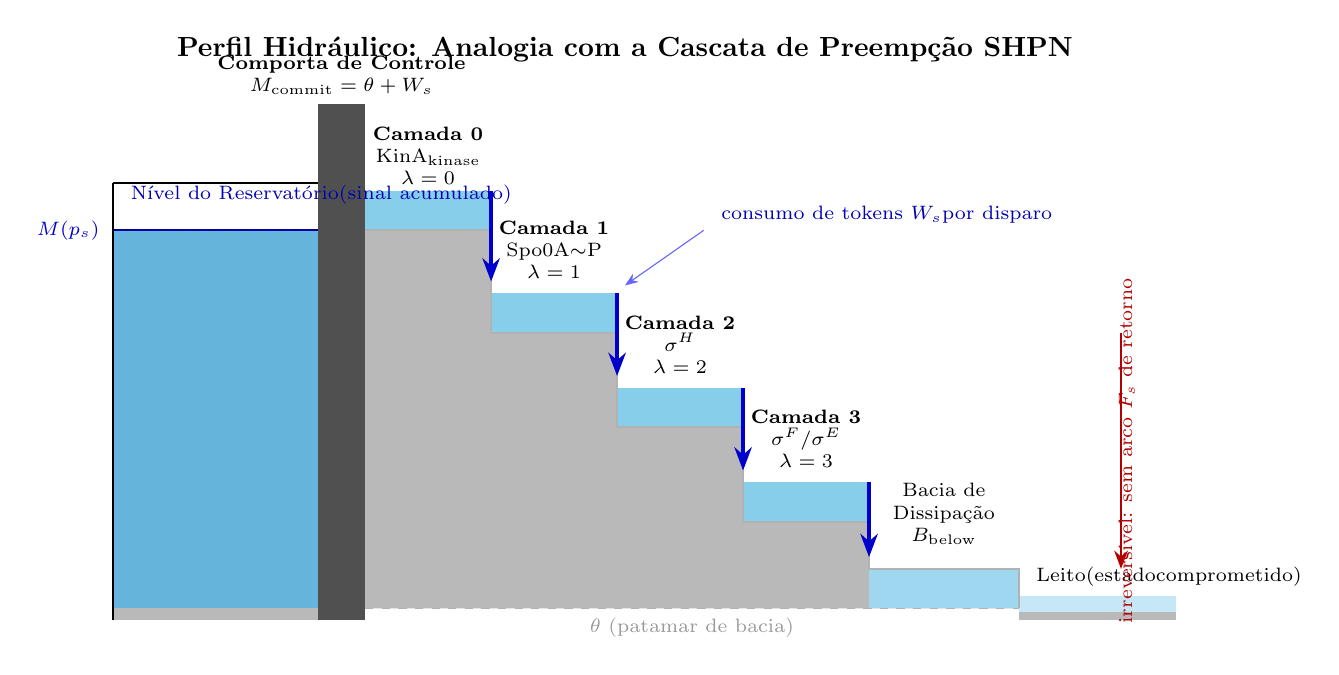
\begin{tikzpicture}[font=\small, >=Stealth]

  %% ── Ground geometry ─────────────────────────────────────────────
  % Reservoir floor
  \fill[gndgray] (0,-0.15) rectangle (2.6,0);
  % Gate block
  \fill[gatecol] (2.6,-0.15) rectangle (3.2,6.4);
  % Stepped ground descending (4 layers + basin)
  \fill[gndgray]
    (3.2,0) -- (3.2,4.8) -- (4.8,4.8) -- (4.8,3.5)
    -- (6.4,3.5) -- (6.4,2.3) -- (8.0,2.3) -- (8.0,1.1)
    -- (9.6,1.1) -- (9.6,0.5) -- (11.5,0.5) -- (11.5,0) -- cycle;
  % River bed
  \fill[gndgray] (11.5,-0.15) rectangle (13.5,0);

  %% ── Reservoir water ─────────────────────────────────────────────
  \fill[waterblue] (0,0) rectangle (2.6,4.8);
  \draw[blue!60!black, thick] (0,4.8) -- (2.6,4.8);
  % reservoir walls
  \draw[thick] (0,-0.15) -- (0,5.4) (0,5.4) -- (2.6,5.4);

  %% ── Water on each step ──────────────────────────────────────────
  \fill[stepwater] (3.2,4.8) rectangle (4.8,5.3);
  \fill[stepwater] (4.8,3.5) rectangle (6.4,4.0);
  \fill[stepwater] (6.4,2.3) rectangle (8.0,2.8);
  \fill[stepwater] (8.0,1.1) rectangle (9.6,1.6);
  % Dissipation basin
  \fill[basinblue] (9.6,0) rectangle (11.5,0.5);
  % River
  \fill[basinblue!60] (11.5,-0.05) rectangle (13.5,0.15);

  %% ── Step outlines ───────────────────────────────────────────────
  \draw[thick, gray!60]
    (3.2,4.8) -- (4.8,4.8) -- (4.8,3.5)
    -- (6.4,3.5) -- (6.4,2.3)
    -- (8.0,2.3) -- (8.0,1.1)
    -- (9.6,1.1) -- (9.6,0.5) -- (11.5,0.5) -- (11.5,0);

  %% ── Cascade flow arrows (at each riser) ─────────────────────────
  \foreach \x/\ytop/\ybot in {%
    4.8/5.3/4.0,
    6.4/4.0/2.8,
    8.0/2.8/1.6,
    9.6/1.6/0.5%
  }{
    \draw[->, very thick, blue!80!black] (\x, \ytop) -- (\x, \ybot+0.15);
  }

  %% ── Gate label ──────────────────────────────────────────────────
  \node[align=center, font=\scriptsize, above] at (2.9,6.4)
    {\textbf{Comporta de Controle}\\
     $M_{\text{commit}} = \theta + W_s$};

  %% ── Reservoir level label ───────────────────────────────────────
  \node[blue!80!black, font=\scriptsize, anchor=east] at (-0.05,4.8)
    {$M(p_s)$};
  \draw[blue!80!black, dashed, thin] (0.05,4.8) -- (2.5,4.8);
  \node[font=\scriptsize, anchor=west, text=blue!70!black] at (0.1,5.25)
    {Nível do Reservatório\\(sinal acumulado)};

  %% ── Layer labels on each tread ──────────────────────────────────
  \node[align=center, font=\scriptsize] at (4.0,5.75)
    {\textbf{Camada 0}\\KinA$_{\text{kinase}}$\\$\lambda=0$};

  \node[align=center, font=\scriptsize] at (5.6,4.55)
    {\textbf{Camada 1}\\Spo0A${\sim}$P\\$\lambda=1$};

  \node[align=center, font=\scriptsize] at (7.2,3.35)
    {\textbf{Camada 2}\\$\sigma^H$\\$\lambda=2$};

  \node[align=center, font=\scriptsize] at (8.8,2.15)
    {\textbf{Camada 3}\\$\sigma^F$/$\sigma^E$\\$\lambda=3$};

  %% ── Basin / committed state ─────────────────────────────────────
  \node[align=center, font=\scriptsize] at (10.55,1.2)
    {Bacia de\\Dissipação\\$B_{\text{below}}$};

  %% ── River / fully committed ─────────────────────────────────────
  \node[font=\scriptsize, anchor=west] at (11.6,0.4)
    {Leito\\(estado\\comprometido)};

  %% ── Token consumption annotation ────────────────────────────────
  \draw[blue!60, thin, ->] (7.5,4.8) -- (6.5,4.1);
  \node[font=\scriptsize, text=blue!70!black, anchor=west] at (7.6,5.0)
    {consumo de tokens $W_s$\\por disparo};

  %% ── Irreversibility annotation ──────────────────────────────────
  \draw[red!70!black, thick, ->] (12.8,3.5) -- (12.8,0.5);
  \node[red!70!black, font=\scriptsize, rotate=90, anchor=south] at (13.1,2.0)
    {irreversível: sem arco $F_s$ de retorno};

  %% ── Theta (basin floor) annotation ─────────────────────────────
  \draw[gray!60, dashed, thin] (3.2,0.0) -- (11.5,0.0)
    node[pos=0.5, below, font=\scriptsize, text=gray!80] {$\theta$ (patamar de bacia)};

  %% ── Title ───────────────────────────────────────────────────────
  \node[font=\normalsize\bfseries] at (6.5,7.1)
    {Perfil Hidráulico: Analogia com a Cascata de Preempção SHPN};

\end{tikzpicture}
\end{document}
